\documentclass[11pt]{article}

\usepackage[T1]{fontenc}
\usepackage[utf8]{inputenc}
\usepackage{lmodern}
\usepackage{amsmath,amssymb,amsthm}
\usepackage{booktabs,tabularx,array,longtable}
\usepackage{graphicx}
\usepackage{caption}
\usepackage{subcaption}
\usepackage{microtype}
\usepackage[round,authoryear]{natbib}
\usepackage{geometry}
\usepackage{xcolor}
\usepackage[hidelinks]{hyperref}
\usepackage[nameinlink,noabbrev]{cleveref}

\hypersetup{
  pdftitle={Stocks Are Not Flows: An Identification Audit of Investor Pressure and Tenure Change in England},
  pdfauthor={Anonymous},
  pdfsubject={Public discussion preprint; structural identification audit of English housing tenure},
  pdfkeywords={housing tenure, private renting, wealth inequality, structural identification, partial identification, reproducible research}
}

\geometry{margin=1in}
\linespread{1.18}
\setlength{\emergencystretch}{3em}
\graphicspath{{../results/gatea/20260801-open-subset-v2/figures/}}

\newtheorem{proposition}{Proposition}
\newtheorem{corollary}{Corollary}
\newtheorem{remark}{Remark}
\newcommand{\col}{\operatorname{col}}
\newcommand{\rank}{\operatorname{rank}}
\newcommand{\R}{\mathbb{R}}
\newcommand{\norm}[1]{\left\lVert #1\right\rVert_2}
\newcommand{\decision}[1]{\texttt{#1}}

\title{\textbf{Stocks Are Not Flows:}\\
An Identification Audit of Investor Pressure and Tenure Change in England}
\author{Anonymous}
\date{1 August 2026\\Public discussion preprint v1.0.0}

\begin{document}
\maketitle

\begin{abstract}
Can a rise in wealthy households' demand for housing explain falling owner
occupation in England? The qualitative mechanism is plausible, but neither its
direction nor its historical contribution is identified by tenure stocks, house
prices, rents, aggregate mortgage rates, and net housing supply alone. We turn an
initial structural project into a prospective identification audit. First, a
source-level novelty review shows that the broad inequality--housing mechanism,
endogenous rent--own--landlord choice, and linked owner-to-landlord flow measures
all have close antecedents. Second, we separate three objects that are often
conflated: tenure stocks, gross property-use transitions, and mechanism-specific
resource flows. Third, a prospectively frozen internal fail-fast design evaluates a 57-moment,
seven-mechanism response system against four deliberately adversarial omitted
mechanisms. The maintained system is locally full rank at all 64 design points,
yet three adversarial profiles exclude zero and required observation maps are
absent. The authorized decision is therefore to stop unique attribution. A
separate deterministic linear-algebra certificate sharpens the diagnosis: after appending
the rival responses, the focal top-resource response lies in their span in both
public and scaled units, so no linear discriminator exists. We then provide a
general sharp-set formulation under bounded nuisance responses and state the
measurement condition that new data must satisfy to break the equivalence. A
hash-pinned public-data layer reproduces seven official series and 43 validation
checks, including an 11.95 percentage-point fall in owner occupation among
households whose reference person is aged 25--44 between 2008--09 and 2018--19.
These accounting facts motivate the question but do not identify its cause. The
paper's contribution is a reproducible framework for publishing a scientifically
useful structural non-identification result and a concrete minimum-data agenda.
\end{abstract}

\noindent\textbf{Keywords:} housing tenure; private renting; wealth inequality;
structural identification; partial identification; reproducibility.\\
\textbf{JEL codes:} C18, C52, R21, R31.

\section{Introduction}

The decline of owner occupation among younger and middle-aged households in
England has invited a compelling narrative. If resources become concentrated at
the top, wealthy households save a larger share, purchase existing housing, and
let it to households priced out of ownership. The same transaction may then
raise the private-rental stock, lower owner occupation, raise prices relative to
rents, and reinforce measured wealth concentration. This narrative links Gary
Stevenson's fixed-asset models to a concrete tenure margin
\citep[esp. pp.~61--62]{stevenson2019}. It is also easy to over-identify.

The empirical difficulty is not that the aggregate trends are invisible. It is
that the objects needed to identify the mechanism differ from the objects in
standard public time series. A tenure share is a stock. An owner-occupied home
sold to a landlord is a gross transition. A wealthy purchaser's incremental
non-housing resources are a mechanism-specific forcing variable. A fall in the
first does not reveal the second, and observing the second does not reveal the
third. Prices create a further simultaneity: housing revaluation raises measured
property wealth, so a contemporaneous wealth share can move because the proposed
outcome moved.

This paper asks a deliberately prior question: \emph{what would have to be
observed, and what restrictions would have to hold, before the historical
contribution of top-resource pressure could be distinguished from middle-resource
loss, credit, rates, supply, taxation, demographics, rental segmentation,
institutional entry, and social-comparison demand?} We answer it with an
auditable sequence rather than a single fitted model.

The sequence has four parts. First, we conduct a source-level novelty gate. The
broad sign pattern is occupied: inequality can lower ownership and raise
price--rent ratios in equilibrium \citep{head2023}; a poor-to-rich resource shift
can induce wealthy portfolio reallocation into housing, higher prices, and lower
rent--price returns \citep{zhang2015}; and top-income growth can instead raise
non-rich housing demand through social comparisons \citep{drechselgrau2026}.
Close quantitative models already include endogenous tenure and household or
institutional landlords \citep{moktan2025,albuquerque2025,cima2026,castellanos2024}.
Moreover, linked Land Registry and rental-listing data have already been used to
classify investor purchases and owner-to-landlord flows
\citep{bracke2021,bankofengland2023flows}. We therefore make no priority claim
for the mechanism, the tenure margin, or the flow concept.

Second, we freeze an ontology and a 57-moment observation schedule before fitting
the expensive model. The focal primitive is a latent aggregate flow of top
non-housing resources, not observed saving, a wealth share, or a housing capital
gain. Direct middle-resource loss and resource-neutral redistribution are separate
experiments. Every synthetic shock has an explicit closure receipt.

Third, we run a fail-fast identification gate. The maintained seven-column
response matrix is full rank at 64 design points, but the more demanding
specificity tests fail. Three of four deliberately constructed rival data-
generating processes produce a nonzero focal profile, and three economically
essential stock-to-observation maps remain unimplemented. The gate stops the
planned structural estimation rather than allowing fit to be mistaken for
identification. A subsequent span calculation shows that the focal response lies
in the admitted nuisance span. This is a deterministic statement about the
synthetic design, not a population false-positive rate or an empirical estimate.

Fourth, we retain what the evidence can support. A public accounting layer
reproduces exact official-source paths, with immutable source hashes, strict
spreadsheet schemas, deterministic figures, and a fresh offline replay. We also
provide a general partial-identification formulation: conditional on a sourced
response set and bounded nuisance contributions, the focal contribution is the
projection of a linear feasibility set and can be computed sharply by two linear
programs. No such empirical response set is presently justified for England, so
we report the method but no historical interval.

The contribution is consequently an identification audit with a value-of-
information result. It is positive in three senses. It separates commonly
conflated estimands; it demonstrates that local full rank can coexist with failure
against omitted mechanisms; and it converts a stopped structural model into a
precise acquisition rule for future data. One well-oriented new measurement can
break a focal--rival equivalence; another stock observation or rescaled version of
the same aggregate series generally cannot.

\section{From Stevenson's thesis to a testable housing claim}
\label{sec:stevenson}

\subsection{What the 2019 thesis establishes}

Stevenson's MPhil thesis studies fixed and reproducible assets in stylised
heterogeneous-agent economies in which asset holdings enter utility
\citep{stevenson2019}. Its central intuition is that a diminishing marginal
propensity to consume can make a resource distribution relevant for the price of
a fixed factor and its effective return. The thesis also recognizes its own
load-bearing preference restriction. When rich households value land itself, the
dynamic model can retain the inequality--price relationship. When they instead
value fungible net worth, reproducible capital and land become direct substitutes
and the steady-state land price collapses to the standard return-arbitrage relation
$p=\rho/r$, independent of the distribution parameter in that exercise
\citep[pp.~48--49]{stevenson2019}.

That negative robustness result is scientifically more informative than a
mechanical extension of the preferred specification. The thesis does not estimate
a tenure transition, observe a landlord purchase, model an empirically disciplined
housing-supply margin, or identify a UK historical contribution. Its final chapter
instead proposes a three-tier extension in which high asset prices may induce a
middle class with small holdings to dissave to the rich
\citep[pp.~61--62]{stevenson2019}. Our project began from
that proposal, but the novelty and identification gates change what can responsibly
be claimed.

\subsection{Why a direct ``three-class model'' is not the residual novelty}

Since 2019, and in some cases before it, adjacent literatures have professionalised
nearly every broad component. Non-homothetic saving links inequality to lower
rates and higher debt \citep{mian2021}; falling rates can in turn affect the upper
tail of wealth \citep{gomez2024}. Housing models contain heterogeneous quality,
search, rent--own choice, household landlords, institutional investors, credit
constraints, and endogenous or fixed construction
\citep{head2023,greenwald2024,cima2026}. Zhang's model is especially close to the
portfolio-pressure story: wealthy households rebalance from bonds into housing
after an inequality shift, while less-resourced non-owners enter later
\citep{zhang2015}. These antecedents validate the economic question but occupy the
generic mechanism.

The residual object is narrower: a transparent test of whether an independently
defined top non-housing resource flow can be distinguished from a direct loss of
middle resources and from named rival mechanisms under England's available
observation map. This object remains useful even when the answer is no. It is not
a claim to be the first study of housing flows: \citet{bracke2021} links transactions
to subsequent rental listings, while the Bank of England classifies owner-to-
landlord, landlord-to-owner, and inter-landlord flows using a longer listing window
\citep{bankofengland2023flows}. Those sources also reveal why a public aggregate
replication is insufficient: the classifications depend on proprietary listing
links, are lagged and revisable, and do not observe purchaser non-housing resources.

\begin{table}[t]
\centering
\caption{Novelty boundary after the source-level gate}
\label{tab:novelty}
\small
\begin{tabularx}{\textwidth}{@{}p{0.24\textwidth}X p{0.25\textwidth}@{}}
\toprule
Object & Closest occupied ground & Permitted residual claim \\
\midrule
Inequality lowers ownership and raises price--rent & Equilibrium sign result in \citet{head2023}; supply-regulation and demand-side rivals & No new sign claim; test distinguishability of a separately defined forcing variable \\
Rich portfolio pressure raises house prices & Fixed-supply heterogeneous-agent mechanism in \citet{zhang2015} & No new mechanism claim; audit top-resource versus middle-resource and rival equivalence \\
Endogenous rent, own, and landlord choice & UK and European structural models including \citet{moktan2025}, \citet{albuquerque2025}, and \citet{cima2026} & No architecture claim; state which observation equations identify which contribution \\
Owner-to-landlord property flows & Transaction--listing links in \citet{bracke2021} and \citet{bankofengland2023flows} & No first-flow claim; distinguish flow classification from purchaser-resource identification \\
Historical England mechanism magnitude & No source located in the bounded review jointly observes the required resource and property-flow objects & Candidate only after an independently sourced response set; currently stopped \\
\bottomrule
\end{tabularx}
\parbox{0.96\textwidth}{\footnotesize
\emph{Notes:} The review establishes collisions and a bounded residual; it is
not proof of worldwide historical priority. Composite novelty by accumulation
of familiar features is not asserted.}
\end{table}

\section{Stocks, gross transitions, and resource contributions}
\label{sec:ontology}

\subsection{The accounting non-equivalence}

Let $O_t$, $L_t$, and $S_t$ denote owner-occupied, privately let, and social or
other housing-use stocks at date $t$. Abstracting temporarily from construction,
demolition, vacancy, and reclassification, the change in privately let stock is
\begin{equation}
  L_t-L_{t-1}=F^{O\rightarrow L}_t-F^{L\rightarrow O}_t.
  \label{eq:stockflow}
\end{equation}
The observed net change does not identify either gross flow. For every $k_t\geq0$,
the pair $(F^{O\rightarrow L}_t+k_t,F^{L\rightarrow O}_t+k_t)$ yields the same
stock path. Adding landlord-to-landlord transactions changes turnover without
changing the tenure stock. New construction, conversions, demolitions, vacancy,
and household--dwelling denominator differences enlarge the equivalence class.

Even a correctly classified $O\rightarrow L$ purchase does not identify the
proposed resource mechanism. The purchaser may be a leveraged household landlord,
an existing cash landlord, a company, an institutional vehicle, or an owner
temporarily letting a former residence. Its finance may reflect current saving,
inheritance, capital gains, mortgage credit, retained rent, or asset substitution.
The resource flow and the property-use transition are therefore distinct latent
coordinates.

\subsection{The focal primitive and closure}

We write $z_T$ for a latent aggregate increment to top non-housing resources and
$z_M$ for a middle-resource primitive. Neither is a contemporaneous wealth share.
Three experiments have different economic meanings:
\begin{align*}
  D1 &: \quad \Delta z_T>0,\quad \Delta z_M=0, \\
  D2 &: \quad \Delta z_T=0,\quad \Delta z_M<0, \\
  E0 &: \quad \Delta z_T=-\Delta z_M>0.
\end{align*}
$D1$ and $D2$ require an explicit external or compositional closure and are
diagnostic derivatives, not closed-economy redistributions. Their derivative sum
represents $E0$ only locally, on the same differentiable equilibrium branch. This
distinction prevents ``pressure from above'' from being defined mechanically as
``impoverishment below.''

The measurement bridge also decomposes a non-housing wealth-stock change into
active accumulation, asset returns, transfers, debt changes, valuation, and
reclassification. Pre-period ranks are fixed locally. Property wealth and housing-
secured debt are excluded from the focal primitive. These restrictions block the
most direct reverse-causality channel but do not create an observed $z_T$ series.

\section{Public evidence and prospectively frozen scope}
\label{sec:data}

\subsection{Source boundary}

The public layer covers an England 2008--2019 core, while retaining each
publisher's stated geography. Seven official sources are pinned by exact URL,
filename, media type, byte ceiling, and SHA-256: English Housing Survey (EHS)
broad tenure, HM Land Registry HPI, separate ONS IPHRP and PIPR rent-index
segments, dwelling stock, components of net housing supply, and Bank of England
quoted mortgage rates \citep{ehs2025,hmlr2026,onsiphrp2025,onspipr2026,
mhclgstock2026,mhclgsupply2025,boequoted2026}. The run rejects unexpected redirects,
hash drift, schema drift, duplicate periods, missing registered support, and
non-positive index or rate domains.

The open subset deliberately omits outputs that need a different assurance tier:
EHS design covariance and fine tenure, Wealth and Assets Survey rank-by-tenure
microdata, an audited Price Paid Data geography concordance, source-backed rival
response sets, and a direct purchaser-resource link. Historical IPHRP and current
PIPR are never level-spliced. The HPI/PIPR ratio is a normalized relative index,
not a landlord yield. Quoted mortgage products are UK offers, not realized England
borrowing costs.

\begin{table}[t]
\centering
\caption{The observation hierarchy and its claim ceiling}
\label{tab:hierarchy}
\small
\begin{tabularx}{\textwidth}{@{}p{0.20\textwidth}p{0.25\textwidth}X@{}}
\toprule
Layer & Example & Maximum interpretation \\
\midrule
Stock & EHS owner and private-renter shares & Current weighted tenure composition; no gross transition \\
Net stock flow & Net additions divided by beginning dwelling stock & Change in the dwelling stock; no purchaser or tenure identity \\
Gross property-use flow & Transaction linked to pre/post rental listing & Classified $O\to L$, $L\to O$, or $L\to L$ transition under a stated window \\
Purchaser finance & Mortgage purpose, cash status, portfolio or legal form & Financing or buyer class; not top non-housing resources \\
Mechanism contribution & Response to an exogenous or bounded resource primitive & Structural or causal contribution only under the corresponding identifying assumptions \\
\bottomrule
\end{tabularx}
\end{table}

\subsection{Previously viewed outcomes and descriptive status}

Feasibility work viewed the EHS endpoints and the 2015--2019 HPI/PIPR endpoint
before the final implementation. These are therefore reproduced accounting facts,
not untouched directional tests. No uncertainty interval is attached to the EHS
age-band shares because the open table does not provide the required survey-design
covariance. The analysis computes shares from unrounded weighted counts and checks
their closure against a common denominator.

\begin{figure}[t]
  \centering
  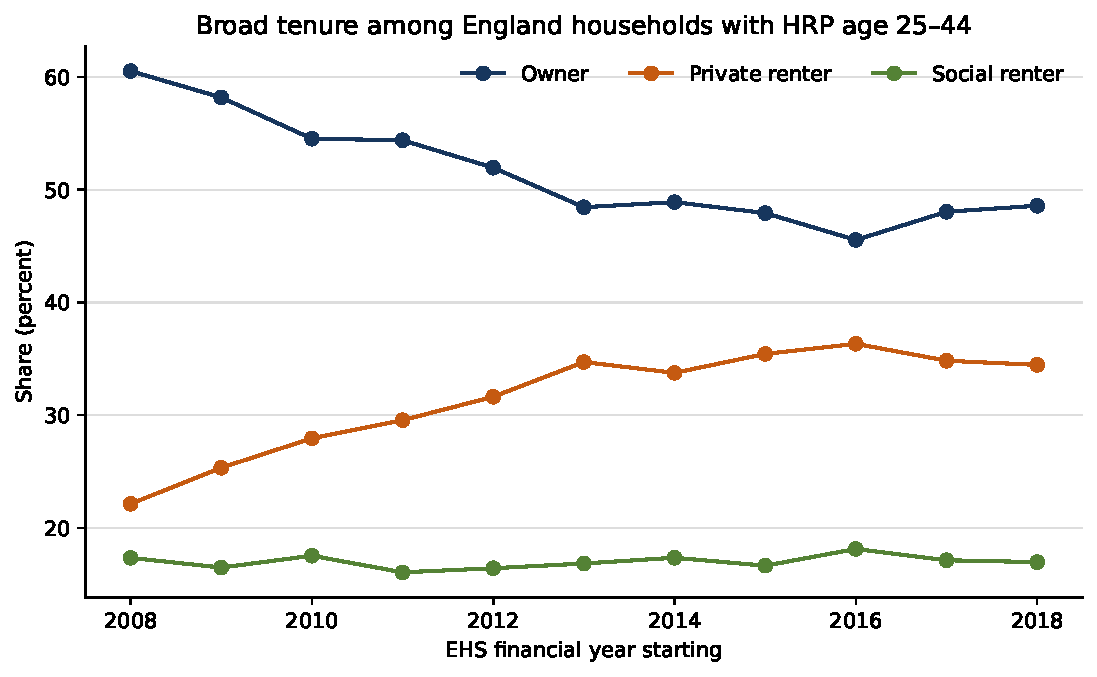
\includegraphics[width=0.84\textwidth]{figure_1_tenure_25_44.pdf}
  \caption{Broad tenure among English households whose household reference
  person is aged 25--44. Points are official weighted estimates reconstructed
  from unrounded counts. The open table does not support design-based confidence
  intervals for the combined age group.}
  \label{fig:tenure}
\end{figure}

Between 2008--09 and 2018--19, the owner share in this population falls from
60.5270\% to 48.5783\%, a change of $-11.9487$ percentage points. The private-
renter share rises from 22.1325\% to 34.4594\%, or $+12.3269$ points; the social-
renter residual changes by $-0.3783$ points. These arithmetic movements are close
to mirror images, but they do not reveal the gross transactions, purchaser types,
or resource origins that produced them.

\begin{figure}[t]
  \centering
  \begin{subfigure}{0.49\textwidth}
    \centering
    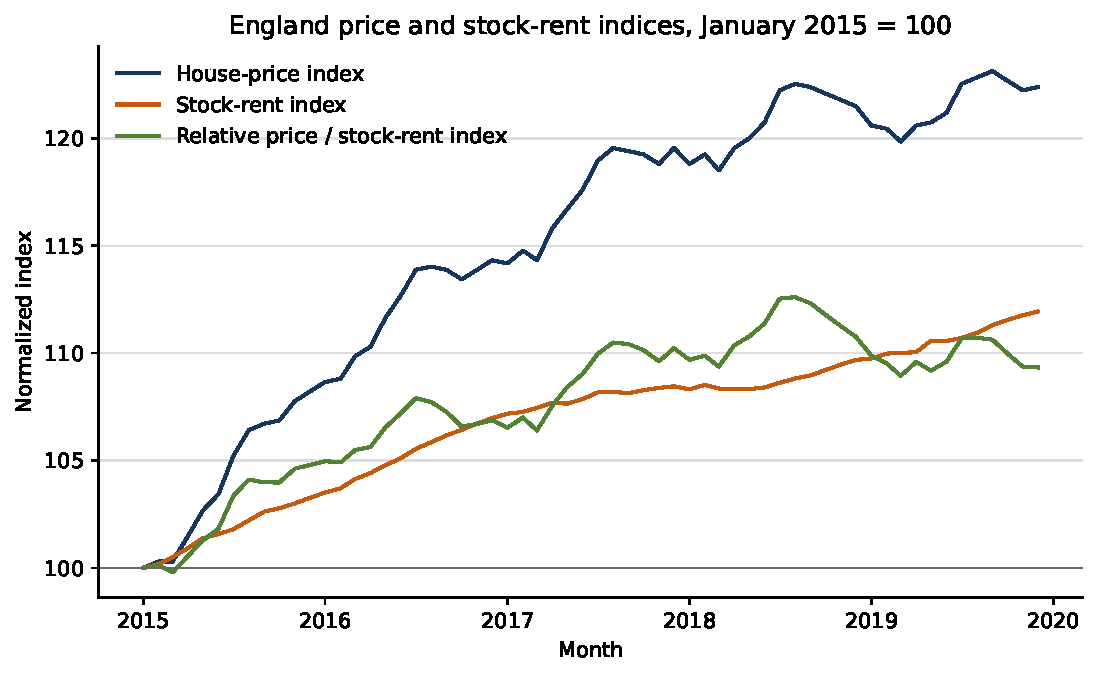
\includegraphics[width=\linewidth]{figure_2_price_stock_rent.pdf}
    \caption{House prices and the separate stock-rent segment.}
  \end{subfigure}\hfill
  \begin{subfigure}{0.49\textwidth}
    \centering
    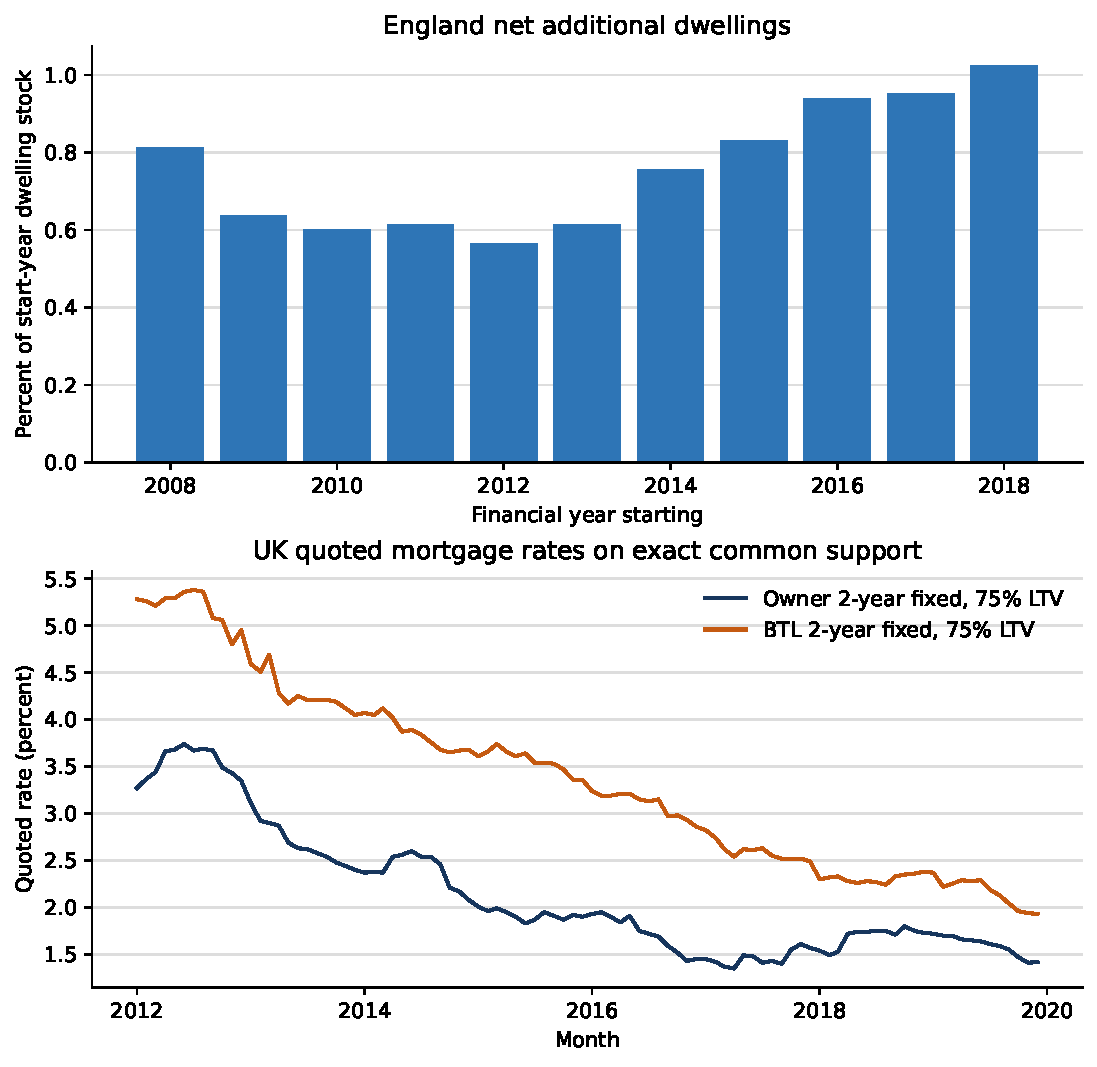
\includegraphics[width=\linewidth]{figure_3_supply_and_rates.pdf}
    \caption{Net additions and quoted mortgage rates.}
  \end{subfigure}
  \caption{Registered public accounting paths. The price-to-stock-rent series
  is normalized in January 2015 and is not a gross or net yield. Mortgage rates
  are quoted UK products; BTL support begins in January 2012.}
  \label{fig:publicpaths}
\end{figure}

The England HPI rises 29.5419\% arithmetically between January 2008 and December
2019. Over their separate registered windows, IPHRP rises 12.6554\% and PIPR
rises 11.9390\%; their levels are not spliced. On matched January 2015--December
2019 support, the normalized HPI-to-PIPR index rises 9.3346\%. Net additions rise
from 0.8119\% to 1.0233\% of the beginning-of-year dwelling stock between the
first and last core years. On January 2012--December 2019 common support, the
mean quoted BTL-minus-owner mortgage spread is 1.2573 percentage points. Each
fact constrains a model, but none is a direct observation of $z_T$.

The Bank's quoted-rate collection changed during 2019 from sampled end-month
observations to whole-market monthly averages. We retain the published series as
a descriptive credit-cost diagnostic and do not interpret the within-series break
as an economic shock.

\section{A fail-fast identification design}
\label{sec:design}

\subsection{Local response map}

Let $g(\theta)\in\R^{57}$ map seven maintained mechanism amplitudes into the
registered target vector, after an explicit public-unit observation adapter. At
a design point $\theta_0$, the local response matrix is
\begin{equation}
  J(\theta_0)=\left[
  \frac{\partial g}{\partial z_T},
  \frac{\partial g}{\partial z_M},
  \frac{\partial g}{\partial c},
  \frac{\partial g}{\partial s},
  \frac{\partial g}{\partial \tau_L},
  \frac{\partial g}{\partial r},
  \frac{\partial g}{\partial d}
  \right],
  \label{eq:jacobian}
\end{equation}
where the remaining columns denote credit, planning or supply, landlord tax,
interest-rate, and demographic blocks. The coefficients are synthetic design
inputs, not empirical elasticities. Percentage-level tenure and pounds-per-week
rent units are preserved before a separately frozen diagonal scaling is applied.

Full column rank of $J$ is necessary for local separation inside the maintained
model but is not sufficient for mechanism specificity. An omitted response can
project onto the focal column even when the maintained columns are linearly
independent. We therefore require known-negative rank controls, deterministic
adversarial data-generating processes, profile diagnostics, and executable maps
between model stocks and aggregate published outcomes before expensive recovery
experiments may run.

\subsection{Prospective decision rule}

The gate was frozen to return either \decision{FAIL-IDENT-0} or
\decision{CONTINUE-TO-FULL-GATE}; it has no path to declare final identification.
A controlling failure stops the 6,573 planned fits and 210,336 optimizer starts.
This is a scientific stop rule, not merely a computational shortcut: once a cheap
test demonstrates that unique attribution is unsupported, running a large model
cannot repair the missing information.

Four deliberately adversarial rival responses represent social comparison,
institutional entry, rental segmentation, and planning restriction. They are
stress constructions, not a random sample of mechanisms. Accordingly, the share
of those four cases producing a nonzero profile is never interpreted as a
population false-positive rate.

\section{Identification geometry and conditional sharp sets}
\label{sec:geometry}

Partition a local linear response as
\begin{equation}
  y=f\beta+N\gamma,
  \label{eq:linearresponse}
\end{equation}
where $f\in\R^m$ is the focal top-resource response, $N\in\R^{m\times k}$ contains
maintained nuisance and admitted rival responses, $\beta$ is the focal amplitude,
and $\gamma$ collects nuisance amplitudes. The following elementary result is the
paper's central diagnostic.

\begin{proposition}[Linear discriminator]
\label{prop:discriminator}
There exists a vector $d\in\R^m$ satisfying $d^{\top}N=0$ and
$d^{\top}f=1$ if and only if $f\notin\col(N)$. When $r=(I-P_N)f\neq0$, where
$P_N$ is the orthogonal projector onto $\col(N)$, one such discriminator is
$d=r/(r^{\top}r)$.
\end{proposition}

\begin{proof}
If $f=Nc$ for some $c$, then every $d$ with $d^{\top}N=0$ also satisfies
$d^{\top}f=d^{\top}Nc=0$, contradicting $d^{\top}f=1$. Conversely, $r$ is
orthogonal to $\col(N)$ and $r^{\top}f=r^{\top}r>0$, so the stated normalization
has both required properties.
\end{proof}

The numerical certificate normalizes each nonzero nuisance column, forms a
truncated-SVD projector, and compares the residual of a unit-norm focal response
with a prospectively fixed tolerance. This makes the span decision invariant to
units without obscuring the original column norms. Repeated time ramps or rescaled
copies of existing moments cannot create a discriminator because they do not add
a new response direction.

Point identification is not the only coherent target. Suppose nuisance
amplitudes have externally justified bounds $\ell\leq\gamma\leq u$, with optional
bounds on $\beta$. The sharp conditional focal set is
\begin{equation}
  \mathcal B(y)=\left\{\beta:\exists\gamma:\;
  y=f\beta+N\gamma,\;\ell\leq\gamma\leq u\right\}.
  \label{eq:identifiedset}
\end{equation}
Because the feasible set is convex, its projection onto $\beta$ is an interval.
Its endpoints solve two linear programs. Infeasibility and unboundedness are
substantive outcomes, not software errors. What gives such an interval empirical
content is the provenance of $f$, $N$, $y$, and the boxes---not the optimizer. The
current England application lacks independently source-backed response sets, so
we do not calculate an empirical interval.

% Results and reproducibility fragment.  The parent document must load booktabs.
% Digests are grouped only to permit line breaking; the rendered hexadecimal
% strings contain no spaces.
\providecommand{\artifactdigest}[8]{{\footnotesize\ttfamily
  #1\allowbreak{}#2\allowbreak{}#3\allowbreak{}#4\allowbreak{}%
  #5\allowbreak{}#6\allowbreak{}#7\allowbreak{}#8}}
\providecommand{\commitdigest}[5]{{\ttfamily
  #1\allowbreak{}#2\allowbreak{}#3\allowbreak{}#4\allowbreak{}#5}}

\section{Results}
\label{sec:results}

The empirical programme was governed by a sequence of stopping rules rather
than by an obligation to produce a structural estimate.  The first rule tested
whether the planned aggregate observation schedule could distinguish a latent
top non-housing resource-flow amplitude, denoted $z_T$ (machine label
\texttt{z\_top}), from six
maintained blocks and four deliberately adversarial omitted mechanisms.  That
test returned \texttt{FAIL-IDENT-0}.  The failure stopped the registered
minimum executable structural model and any unique historical attribution.
We therefore report three objects with different evidential status: the
authoritative IDENT-0 design diagnostic, a licence-safe reproduction of an
open public-accounting subset, and a deterministic design-geometry
certificate.  None is a causal estimate of wealth-driven tenure change.

\subsection{IDENT-0: local rank without mechanism specificity}
\label{sec:ident0-results}

The authoritative v2 run adapted all 57 registered targets to their declared
public units and assigned a unique valid accounting receipt to each of 313
closure cases.  The maintained seven-column response matrix passed the local
rank front at all 64 design points and at each of three central-difference step
sizes.  Across those evaluations, the scaled condition number ranged from
$62.3556$ to $64.0830$.  The known-negative controls behaved as registered:
exact top--middle collinearity reduced rank from seven to six, near
collinearity raised the condition number above $3.418\times10^{8}$, and an
exact top mimic was detected.

These checks establish that the restricted maintained design is numerically
non-degenerate; they do not establish specificity.  In the adversarial part of
the harness, three of four deliberately constructed omitted-mechanism cases
induced a $z_{\mathrm{top}}$ profile that excluded zero when fit by the
restricted seven-block model.  This is a deterministic stress-harness result,
not a population frequency or a false-positive rate.  In none of the four
cases was $z_{\mathrm{top}}$ co-largest in absolute value, and all 32 starts in
each case converged to the same basin.  The three missing observation maps---
owner and landlord prices to aggregate HPI, dwelling stocks to household
tenure, and lifecycle states to the age-25--44 population---were independent
reasons to fail the gate.  Table~\ref{tab:ident0-criteria} records the
controlling criteria.

\begin{table*}[t]
  \centering
  \caption{Authoritative IDENT-0 v2 criteria.}
  \label{tab:ident0-criteria}
  \small
  \begin{tabular}{@{}p{0.255\textwidth}cp{0.255\textwidth}p{0.355\textwidth}@{}}
    \toprule
    Criterion & Status & Registered threshold or control & Realised value and interpretation \\
    \midrule
    Public-unit observation schedule
      & Pass & 57 targets adapted; no pending adapter
      & 57 targets; H05 retained as an explicit non-modelled holdout. \\
    Signed closure coverage
      & Pass & One unique, valid receipt for every case
      & 313/313 cases, using the registered elementary, composite-open, or no-change taxonomy. \\
    Maintained local identification
      & Pass & At least 61/64 rank-seven points; midpoint must pass
      & 64/64 points passed at all three step sizes; scaled condition numbers $62.3556$--$64.0830$. \\
    Exact- and near-collinearity controls
      & Pass & Exact mutation must lose rank; near mutation must exceed $10^{4}$
      & Exact ranks $6,6,6$; near-collinear condition numbers approximately $3.418\times10^{8}$. \\
    Constructed-rival zero-profile diagnostic
      & Fail & No more than 0.05 of the four registered profiles may exclude zero
      & 3/4 profiles excluded zero.  This proportion describes four constructed cases only. \\
    Constructed-rival top-largest diagnostic
      & Pass & No more than 0.10 may make $z_{\mathrm{top}}$ co-largest
      & 0/4 cases made $z_{\mathrm{top}}$ co-largest. \\
    Constructed-rival optimiser stability
      & Pass & At least 30/32 starts per case in the same basin
      & 32/32 for each of four cases. \\
    Exact top-mimic detection control
      & Pass & Harness must expose attribution under identical labels
      & The control returned $\widehat z_{\mathrm{top}}=0.65$ and profile $[0.375,0.925]$. \\
    Three observation bridges
      & Fail & Each bridge must be executable
      & All three were \texttt{NOT\_IMPLEMENTED}: HPI aggregation, dwelling-to-household tenure, and age-25--44 lifecycle aggregation. \\
    \bottomrule
  \end{tabular}
  \parbox{0.96\textwidth}{\footnotesize
    Notes: the machine report contains 12 criteria in total: eight pass and
    four fail.  The final row consolidates three separately recorded failures.
    Synthetic response coefficients, terminal wealth loadings, and diagonal
    scales are recovery-design inputs, not empirical elasticities or sampling
    standard errors.}
\end{table*}

Because the fail-fast front was decisive, the precomputed full-stage workload
of 6,573 fits and 210,336 optimiser starts was not run.  In particular, the
313-case recovery aggregation, noisy-fit coverage and classification checks,
64-case profile aggregation, rival-compensation tests, outer optimiser rule,
structural mutations, and the P5 landlord-yield signature remain unexecuted.
The run did not issue, and could not be read as issuing, a pass for unique
attribution.

\subsection{Gate A: reproduced public accounting, with the full gate held}
\label{sec:gatea-results}

After the identification stop, Gate A was restricted to deterministic
accounting over seven official public sources.  All seven downloaded objects
matched their prospectively frozen SHA-256 digests, and all 43 schema, support,
closure, and arithmetic checks passed.  This produced nine derived tables and
three figures in PDF and SVG.  Its only authorised success label was
\texttt{OPEN-SUBSET-REPRODUCED+FULL-GATE-A-HELD}; the runner had no code path
to authorise structural estimation, unique attribution, or causal language.

For private households in England whose household reference person was aged
25--44, the open English Housing Survey table gives an owner point estimate of
$60.5270\%$ in 2008--09 and $48.5783\%$ in 2018--19, a change of
$-11.9487$ percentage points (Table~\ref{tab:accounting-facts}).  The private-
renter estimate moved from $22.1325\%$ to $34.4594\%$, or $+12.3269$
percentage points; the social-renter estimate changed by $-0.3783$ percentage
points.  These shares were recomputed from unrounded weighted counts over a
common denominator.  The maximum discrepancy from published age-specific
percentages was $1.99\times10^{-13}$ percentage points, and the largest
absolute three-tenure closure residual was $2.84\times10^{-13}$ percentage
points.  The public table supplies neither the design covariance needed for
joint inference nor the registered fine-tenure categories, so these are point
estimates without confidence intervals.

The England all-property HPI rose from 63.3 in January 2008 to 82.0 in
December 2019, an endpoint change of $29.5419\%$ (or $25.8834$ log points).
The historical IPHRP stock-rent segment rose $12.6554\%$ over 2008--2014, and
the methodologically separate PIPR segment rose $11.9390\%$ over 2015--2019.
Those levels were not spliced.  On their common 2015--2019 support, normalising
both HPI and PIPR to January 2015 yields a price-to-stock-rent relative index
that rose $9.3346\%$; its reciprocal fell $8.5377\%$.  This relative index is
not a gross or net rental yield.

Net additions increased from $0.8119\%$ of the start-of-year dwelling stock in
2008--09 to $1.0233\%$ in 2018--19.  The denominator is all dwellings,
including vacant dwellings, and is not interchangeable with the household
denominator used for tenure.  The maximum absolute residual between the
published net-additions total and its components was 13 dwellings, below the
pre-run quality-control tolerance of 50.  Finally, on the 96-month common
support from January 2012 to December 2019, the quoted two-year fixed 75\% LTV
buy-to-let minus owner-occupier mortgage-rate spread declined from 2.01 to
0.51 percentage points and averaged 1.2573 points.  These are United Kingdom
quoted product rates, not realised borrowing costs for English households.  The
publisher's 2019 change from sampled end-month observations to whole-market
monthly averages is a measurement break, so the series is retained only as a
descriptive diagnostic rather than interpreted as a policy or market shock.

\begin{table*}[t]
  \centering
  \caption{Reproduced Gate A public-accounting facts.}
  \label{tab:accounting-facts}
  \small
  \begin{tabular}{@{}p{0.215\textwidth}p{0.335\textwidth}p{0.365\textwidth}@{}}
    \toprule
    Registered fact & Reproduced accounting result & Interpretation ceiling \\
    \midrule
    AF01: owner tenure, HRP 25--44
      & $60.5270\%$ (2008--09) to $48.5783\%$ (2018--19); $-11.9487$ percentage points
      & England point estimates; public design covariance unavailable. \\
    AF02: private renting, HRP 25--44
      & $22.1325\%$ to $34.4594\%$; $+12.3269$ percentage points
      & Same household denominator and uncertainty restriction as AF01. \\
    AF03: broad-tenure path
      & 11 financial years, 2008--09 to 2018--19; owner/private/social only
      & Fine tenure and joint covariance remain EUL-blocked. \\
    AF07: England HPI
      & 63.3 (January 2008) to 82.0 (December 2019); $+29.5419\%$
      & Unadjusted all-property index; not a landlord-specific price. \\
    AF08: stock-rent segments
      & IPHRP $+12.6554\%$ (2008--2014); PIPR $+11.9390\%$ (2015--2019)
      & Separate method segments; no level splice. \\
    AF09: normalised price/stock-rent index
      & $+9.3346\%$ over January 2015--December 2019; reciprocal $-8.5377\%$
      & A relative index, not a rental yield. \\
    AF11: net additions rate
      & $0.8119\%$ (2008--09) to $1.0233\%$ (2018--19)
      & Flow divided by start-of-year all-dwelling stock, including vacant dwellings. \\
    AF12: quoted mortgage-cost diagnostic
      & 96 common months; BTL-minus-owner spread 2.01 to 0.51 points; mean 1.2573
      & UK quoted offers, not realised England borrower costs. \\
    \bottomrule
  \end{tabular}
  \parbox{0.96\textwidth}{\footnotesize
    Notes: EHS endpoints and the 2015--2019 HPI/PIPR endpoint had been viewed
    during feasibility work.  Their manifest-bound calculation is therefore a
    reproduction of previously observed accounting facts, not an untouched
    directional confirmation.  Passing arithmetic checks authenticates the
    registered transformation; it does not validate a causal mechanism.}
\end{table*}

Full Gate A remains held.  The open EHS table lacks design covariance and fine
tenure; net non-housing wealth by rank and tenure requires Wealth and Assets
Survey EUL microdata; the Price Paid Data turnover module requires an audited
England/Wales concordance; and source-backed rival response sets remain absent.
The FCA mortgage table and the English Private Landlord Survey are bounded
extensions rather than inputs to this run.  Most importantly, the unrestricted
open core does not jointly label gross property-use transitions, purchaser
landlord identity, and purchaser top non-housing resources.  Existing
proprietary and safeguarded listing linkages remain relevant prior evidence;
their existence also precludes any claim that property-use flows have never
been measured.

\subsection{Partial identification: a design-geometry obstruction}
\label{sec:partialid-results}

The post-gate certificate asks whether the focal response column has a
component outside the span of the other six maintained columns and the four
admitted rival signatures.  Within the maintained 57-by-7 matrix, rank is
seven in both public units and the prospectively frozen synthetic diagonal scaling.
After adding four rival columns, the 57-by-11 matrix has rank nine.  Projection
of the focal $z_{\mathrm{top}}$ column onto the ten nuisance and rival columns
leaves relative residuals of $1.461\times10^{-14}$ in public units and
$2.323\times10^{-14}$ after synthetic scaling, both far below the registered
$2\times10^{-10}$ effective tolerance (Table~\ref{tab:geometry-certificate}).
No dual discriminator exists at that tolerance.

\begin{table}[t]
  \centering
  \caption{Partial-identification design-geometry v1 certificate.}
  \label{tab:geometry-certificate}
  \small
  \begin{tabular}{@{}lrrrr@{}}
    \toprule
    Basis & Maintained rank & Condition no. & Augmented rank & Relative residual \\
    \midrule
    Public units & $7/7$ & $68.8814$ & $9/11$ & $1.46097\times10^{-14}$ \\
    Synthetic scaling & $7/7$ & $63.3405$ & $9/11$ & $2.32265\times10^{-14}$ \\
    \bottomrule
  \end{tabular}
  \parbox{0.94\columnwidth}{\footnotesize
    Notes: columns are individually normalised for the span calculation.  The
    maximum absolute difference between the analytic public-unit derivative
    and its central-difference control was $1.34432\times10^{-9}$.  The
    augmented condition number is intentionally not reported because the
    augmented matrix is rank-deficient.}
\end{table}

The certificate decision is
\texttt{STOP-UNIQUE+GO-PARTIAL-ID-THEORY}.  It reconciles two facts that would
otherwise appear contradictory: the focal coefficient is locally recoverable
inside the restricted maintained matrix, yet is not identified against the
enlarged admitted span.  This is a deterministic algebraic statement about
the supplied columns.  All maintained loadings, baselines, scales, and rival
signatures are synthetic design inputs, and the four rivals are constructed
stress cases rather than draws from any population.  No response set in this
certificate has been independently source-backed or transported to England.
Consequently, the certificate supplies neither an England elasticity nor an
empirical interval for the historical contribution of top resources.

The accompanying linear-programming layer can compute a sharp interval for a
focal coefficient conditional on an observed response equation and declared
box restrictions on nuisance coefficients.  Promotion of such an interval to
an empirical England bound would require independently sourced mechanism
response sets, explicit geography/time/population/unit transport sets, and
sensitivity to enlarging the rival set and relaxing its boxes.  Those inputs
do not yet exist, so no numerical England contribution bound is reported.

\clearpage

\section{Reproducibility and assurance}
\label{sec:reproducibility}

\subsection{Immutable run identities}

Every reported run required a clean Git worktree and recorded the command,
commit, configuration and source-code digests, Python platform, NumPy and SciPy
versions, and the fixed provenance seed 20260801.  IDENT-0 v2 ran at commit
\commitdigest{1e04a181}{78310505}{1c819af1}{90b95463}{40bbb1fd}; Gate A v2, its offline
replay, and the partial-ID certificate ran at commit
\commitdigest{836e3391}{355f8443}{8af0d321}{f69e9428}{1050c00d}.  The authoritative identities
are:

\begin{table*}[t]
  \centering
  \caption{Manifest- and report-bound run identities.}
  \label{tab:run-identities}
  \small
  \begin{tabular}{@{}p{0.18\textwidth}p{0.345\textwidth}p{0.345\textwidth}@{}}
    \toprule
    Run & Manifest SHA-256 & Report SHA-256 \\
    \midrule
    IDENT-0 v2
      & \artifactdigest{a23d17ea}{471eb7ed}{67a96e34}{b5fb85f7}{c50b34c7}{e2319874}{98ed3696}{3220ccda}
      & \artifactdigest{049ec5f8}{c3e290d1}{c0273c86}{30e3c8d1}{eeee8c21}{91427fcd}{97428030}{60bfca35} \\
    Gate A v2, online
      & \artifactdigest{3e1f92e4}{36e3744d}{6702d831}{4c9f4c0f}{5602898d}{5b996f9a}{60fa0010}{af291c90}
      & \artifactdigest{97925770}{879ca8f9}{e356c067}{c9d9c6b4}{b98d5d09}{81133544}{85002bed}{8bcc2f08} \\
    Gate A v2, offline replay
      & \artifactdigest{f00bfcac}{e904d7a3}{cb6fcb87}{46d1fb03}{46b38e74}{de6d6722}{4d868ccb}{0a03a57b}
      & \artifactdigest{51aa01e7}{a0b2fe14}{aed73e3d}{3ff43b53}{3637f1e4}{3f91a0bc}{96598ef5}{4f1cc530} \\
    Design geometry v1
      & \artifactdigest{7e76a293}{0297e0b1}{3ad2cd6a}{a1a6a4a4}{3cbe0a47}{8da24050}{11a30fad}{baf51b5d}
      & \artifactdigest{421ce83b}{335bf610}{e2f7fa3c}{fb178b6a}{2ebc7620}{098d05b9}{f5601d16}{4cb1d7fc} \\
    \bottomrule
  \end{tabular}
\end{table*}

The seven official Gate A source objects were also pinned before extraction
(Table~\ref{tab:source-digests}).  A matching digest establishes byte identity
with the registered source object; it does not establish survey validity,
measurement accuracy, or a causal interpretation.

\begin{table*}[t]
  \centering
  \caption{Registered source-object digests for Gate A v2.}
  \label{tab:source-digests}
  \scriptsize
  \begin{tabular}{@{}p{0.29\textwidth}p{0.58\textwidth}@{}}
    \toprule
    Source object & SHA-256 \\
    \midrule
    EHS FA1201 open table
      & \artifactdigest{f095268b}{6330ec5e}{4733b047}{4f53d8b7}{9d7a6932}{dc939e0b}{65196799}{d54252ac} \\
    HM Land Registry HPI indices, May 2026
      & \artifactdigest{cacaef81}{b8f09c0b}{1c67c9a8}{a7c07713}{4384a1be}{4dd1b1dd}{f26a9c52}{656620a5} \\
    ONS historical IPHRP time series, version 25
      & \artifactdigest{bf87cfd2}{93323df5}{c558a203}{635d69c1}{6b9b1c48}{485d410a}{fc19563c}{016228f1} \\
    ONS PIPR workbook, 22 July 2026
      & \artifactdigest{d429e553}{ade45490}{3b731f6c}{257609f1}{4d0c2171}{822791e0}{9c21a9d5}{3d5e24a9} \\
    MHCLG dwelling stock Live Table 104
      & \artifactdigest{ecd02eb8}{e520e4fe}{f7878bda}{35db002c}{a2360cb4}{5112416d}{b6619863}{b211a1fa} \\
    MHCLG net supply Live Table 120
      & \artifactdigest{548101e5}{35b7db4e}{0718a1ef}{3129e343}{169cb398}{2f1cd8e0}{3c0f247e}{93c5d219} \\
    Bank of England quoted-rate extract
      & \artifactdigest{d5c17cab}{c1103c33}{96695f38}{9c6384b7}{45ce58e8}{f4f07787}{f83d82a6}{2127f009} \\
    \bottomrule
  \end{tabular}
\end{table*}

\subsection{Online acquisition and offline replay}

Gate A v2 was first run against the registered official HTTPS locations and
then rerun using only the immutable raw directory from the online run.  The
seven raw files, all nine derived CSVs, all six rendered figure files, and
\texttt{TABLE\_METADATA.json} were byte-identical across the two runs.  The
scientific content of \texttt{REPORT.json} was also identical after excluding
its run-manifest digest.  The complete report and directory digests differ by
design: the online and offline manifests record different commands, and their
source receipts record official-HTTPS retrieval versus offline-cache replay.
This is therefore an exact replay of the pinned scientific payload, not a claim
that provenance-bearing directories are byte-for-byte identical.

From the repository root, the manifest-recorded commands (with the local
virtual-environment prefix shortened to \texttt{.venv/bin}) are:

\begin{quote}
\footnotesize\ttfamily
.venv/bin/housing-ident0 --config configs/ident0.json\par
\quad --output-dir results/ident0/20260801-ident0-failfast-v2\par
\quad --exit-zero-on-scientific-fail\par\medskip
.venv/bin/housing-gatea --config configs/gatea\_public.json\par
\quad --output-dir results/gatea/20260801-open-subset-v2\par\medskip
.venv/bin/housing-gatea --config configs/gatea\_public.json\par
\quad --offline-source-dir results/gatea/20260801-open-subset-v2/raw\par
\quad --output-dir results/gatea/20260801-open-subset-v2-replay\par\medskip
.venv/bin/housing-partialid --config configs/ident0.json\par
\quad --ident0-report results/ident0/20260801-ident0-failfast-v2/REPORT.json\par
\quad --output-dir results/partialid/20260801-design-geometry-v1
\end{quote}

The IDENT-0 option \texttt{--exit-zero-on-scientific-fail} changes only the
shell exit status used by the release workflow; it does not change the
\texttt{FAIL-IDENT-0} decision written into the report.  The Gate A downloader
fails closed on host, media-type, byte-ceiling, schema, support, and digest
drift.  Scientific invariants use explicit exceptions rather than Python
\texttt{assert}, and the focused test protocols include optimised
\texttt{python -O} execution so that disabling assertions cannot erase those
checks.

\subsection{Assurance boundary and remaining work}
\label{sec:assurance-boundary}

The combined evidence supports three deliberately narrow conclusions.  First,
the prospectively frozen aggregate design does not support unique attribution of
England's tenure change to the focal resource mechanism once the registered
adversarial rivals and missing observation bridges are taken seriously.
Second, a bounded collection of public tenure, price, rent, housing-supply, and
quoted-rate paths is reproducible from pinned official bytes.  Third, within
the synthetic design harness, the focal response lies in the enlarged nuisance
and rival span at the registered numerical tolerance.

It does not support a causal top-wealth-to-tenure claim, a historical
contribution percentage, a general-equilibrium result, an empirical England
elasticity, or an England partial-identification interval.  Hashes authenticate
the bytes and declared replay boundary, not the correctness of publisher
methods or the truth of an economic mechanism.  Deterministic replay is not
independent replication.  Likewise, agreement between an analytic derivative
and a finite-difference control validates an implementation detail, not its
empirical calibration.

An empirical promotion would require, at minimum, survey-design covariance and
fine-tenure microdata; net financial plus business wealth by resource rank and
tenure; an audited map between dwelling flows and household tenure; direct or
defensibly bounded purchaser-resource information; and independently
source-backed response sets for every admitted mechanism with explicit
transport across geography, period, population, unit, and scale.  Until those
conditions are met, the appropriate endpoint is the present identification
audit and public-accounting package, with \texttt{STOP-UNIQUE} and
\texttt{STOP-CAUSE} retained.

\clearpage


\section{Minimum-data and value-of-information result}
\label{sec:min-data}

The failed gate does more than request ``better data.'' It specifies the direction
that a useful measurement must add. Let $C=\{c:Nc=f\}$ be the set of nuisance
representations of the current focal response. Append one new measurement with
focal response $a_f$ and nuisance row $a_N^{\top}$. The extended columns are
\[
  f^+=\begin{bmatrix}f\\a_f\end{bmatrix},\qquad
  N^+=\begin{bmatrix}N\\a_N^{\top}\end{bmatrix}.
\]

\begin{proposition}[A measurement that breaks observational equivalence]
\label{prop:newmeasurement}
If $f\in\col(N)$ in the current observation map, then the appended measurement
identifies a new focal direction if and only if
\begin{equation}
  a_f\notin\{a_N^{\top}c:c\in C\}.
  \label{eq:newrow}
\end{equation}
Equivalently, $f^+\notin\col(N^+)$. Thus one well-oriented scalar measurement can
be sufficient, while arbitrarily many measurements satisfying the same nuisance
representation cannot help.
\end{proposition}

\begin{proof}
$f^+\in\col(N^+)$ precisely when there exists $c$ such that both $Nc=f$ and
$a_N^{\top}c=a_f$. This is equivalent to $a_f$ belonging to the set on the
right-hand side of \cref{eq:newrow}. Negating the condition and applying
\cref{prop:discriminator} gives the result.
\end{proof}

The synthetic augmented matrix has 11 columns and rank nine, but its two-
dimensional algebraic rank deficit is not a claim that exactly two real-world
variables are required. The orientation of a measurement matters more than its
count. In housing terms:
\begin{enumerate}
  \item another tenure-stock year, or the same stock expressed in a different
  denominator, is unlikely to break the equivalence;
  \item a validated $O\rightarrow L$ transaction label reduces gross-flow
  ambiguity but still does not reveal the purchaser's resource shock;
  \item a top non-housing wealth measure without a property linkage remains
  vulnerable to asset returns, transfers, debt changes, and aggregation; and
  \item the most valuable design jointly links pre-determined non-housing
  resources or a defensible resource shock to purchaser identity, property-use
  transition, financing, and a comparison group, with supply and credit responses
  measured on compatible support.
\end{enumerate}

This joint object could arise from securely linked tax, mortgage, ownership, and
rental-listing records, or from a narrowly valid policy or windfall design. Access
alone is not identification: linkage error, anticipation, legal-form switching,
reclassification, and equilibrium spillovers must enter the response set. The
criterion in \cref{eq:newrow} provides a pre-analysis value-of-information test for
candidate acquisitions.

\section{Discussion}
\label{sec:discussion}

\subsection{What the failure establishes}

The results establish that the registered synthetic observation map does not
support unique top-resource attribution. This conclusion is stronger than noting
that a regression may be endogenous and weaker than proving that no conceivable
England design can identify the mechanism. It is bound to the admitted response
class. A new source or restriction can alter the column space; it must be justified
without using the desired conclusion.

Local full rank and low residual loss inside a maintained model should therefore
not be reported as identification when omitted economically plausible mechanisms
have aligned responses. The known-negative controls in this project illustrate
the difference: the code correctly rejects exact and near collinearity, yet the
apparently healthy seven-column design remains non-specific after rivals are
admitted. The problem is semantic coverage, not numerical optimization.

\subsection{What the public facts do and do not show}

The open data show a large reallocation of broad tenure among households aged
25--44, rising house prices, rising stock rents, changes in relative prices, a
recovering net-supply rate, and a narrowing quoted BTL mortgage spread over the
registered window. These are important constraints. They do not determine
whether the tenure shift arose from rich household purchases, institutional entry,
middle-resource loss, credit conditions, supply, demographics, or combinations.
Nor can the near-offsetting owner and private-renter share changes be treated as
gross owner-to-landlord transfers.

The linked-listing literature is informative but does not close the mechanism.
\citet{bracke2021} defines investor acquisition through a rental listing within six
months of sale. The later Bank measure uses a four-year window and prior/subsequent
listing histories to classify three property flows
\citep{bankofengland2023flows}. These are different estimands; both are sensitive
to coverage, timing, and classification; online-listing volume is itself sensitive
to platform coverage \citep{livingston2021}. Neither directly identifies purchaser
wealth rank or the origin of funds. A future paper should treat their definitions
as measurement models, not ground-truth labels.

\subsection{Relation to partial identification}

Partial identification is not a rhetorical downgrade of point identification.
It replaces a false singleton with a transparent set whose width reflects admitted
uncertainty \citep{manski2003,tamer2010}. The sharp-set machinery in this paper is
ready to accept source-backed mechanism response ranges. It deliberately refuses
to transform the synthetic IDENT-0 loadings into an England interval. Informative
bounds may eventually support a near-zero, signed, or sign-ambiguous conclusion;
all are scientifically admissible.

\subsection{Limitations}

Four limitations define the paper's claim ceiling. First, the public tenure path
contains point estimates without the design covariance needed for combined-age
inference. Second, the design responses and adversarial rivals are synthetic.
They test a planned model, not England. Third, the novelty search is bounded and
cannot prove global priority. Fourth, the analysis does not estimate a causal or
structural historical contribution. These limitations are not buried robustness
notes: they determine the title, abstract, and decision code.

\section{Conclusion}

The project began with an intuitively attractive extension of Stevenson's thesis:
wealth concentration raises fixed-asset demand, encourages middle-class dissaving,
and reallocates owner-occupied homes to landlords. The novelty gate showed that
the broad theoretical and empirical territory is already occupied. The
identification gate then showed that the registered aggregate observation map
cannot distinguish the focal top-resource response from admitted alternatives.
The responsible outcome is not to force a structural estimate. It is to publish
the boundary.

Three results survive that boundary. Official public data reproducibly document
the motivating accounting paths. A discriminator theorem and manifest-bound
certificate state exactly why unique attribution fails in the planned design. A
conditional sharp-set framework and new-measurement criterion turn the failure
into a concrete data-acquisition agenda. In this setting, ``stocks are not flows''
is not merely a warning about terminology. It is the identification result.

\section*{Declarations}

\paragraph{Data and code availability.}
The replication package contains source identities and hashes, extraction and
validation code, tests, machine-readable reports, deterministic figures, and a
deterministic offline replay. Restricted, safeguarded, proprietary listing, and
address-level data are not redistributed. Exact release identifiers are reported
in the reproducibility appendix. The archival preprint and replication package
are at \href{https://doi.org/10.5281/zenodo.21740339}{doi:10.5281/zenodo.21740339};
the public source repository is
\url{https://github.com/ipitchford/stocks-are-not-flows}.

\paragraph{Internal protocol and outcome viewing.}
The public pilot was governed by a prospectively frozen internal protocol and
three amendments. The EHS
endpoints and the 2015--2019 HPI/PIPR endpoint had been viewed during feasibility
work. The net-supply component tolerance was fixed during pre-run schema
inspection. These disclosures preclude an untouched confirmatory interpretation.

\paragraph{Competing interests and funding.}
No funding or competing-interest declarations were supplied for this anonymous
public discussion preprint. These declarations, affiliations, and accountable
human authorship must be completed before journal submission.

\paragraph{Use of computational assistance.}
Automated research and coding tools assisted source discovery, implementation,
testing, and manuscript drafting. Human authors remain responsible for source
verification, the scientific claims, and the submitted text. Automated tools are
not authors.

\appendix
% Self-contained notation; include this file after \appendix in the main paper.
\section{Identification and stock--flow accounting results}
\label{app:identification-theory}

\subsection{Scope, novelty, and assurance boundary}
\label{app:scope}

This appendix states the mathematical results used to interpret the empirical
design. The rank identities, projection arguments, linear-programming
characterisation, and stock--flow inequalities below are standard consequences
of finite-dimensional linear algebra, convex analysis, and accounting. We do
not claim them as new theorems. The housing-specific contribution is instead
the disciplined application of these results to a prospectively frozen observation
map, the separation of stocks from gross flows, and the use of explicit
response sets and provenance gates before attaching an empirical
interpretation.

Nothing in this appendix supplies a numerical bound for England. In
particular, a response column used in a design audit is not thereby established
as a historical response, a causal impulse response, or a transportable
elasticity. Any empirical interval requires independently sourced response
sets, declared population and time transport assumptions, and a separate
measurement audit. The propositions below describe what follows
\emph{conditional on} their stated matrices and restrictions.

\subsection{Linear response setup}
\label{app:linear-setup}

Let \(y\in\mathbb R^m\) denote an observed vector of moments. The exact linear
response model is
\begin{equation}
  y=f\beta+N\gamma,
  \label{eq:linear-response}
\end{equation}
where \(f\in\mathbb R^m\) is the response column for the focal mechanism,
\(\beta\in\mathbb R\) is its coefficient,
\(N\in\mathbb R^{m\times k}\) collects admitted nuisance and rival response
columns, and \(\gamma\in\mathbb R^k\) contains their coefficients. Zero or
linearly dependent columns of \(N\) are allowed. Unless restrictions are
introduced explicitly, \(\gamma\) is unrestricted.

The phrase \emph{identified against the admitted span} is deliberate. It is a
statement about the columns included in \(N\), not a guarantee that all
economically relevant mechanisms have been included. Enlarging \(N\) can
remove identification; validating the membership of \(N\) is therefore a
substantive part of the empirical design rather than a purely numerical step.

\subsection{A common time path cannot create a new identifying direction}
\label{app:common-path}

Suppose \(a_j\in\mathbb R^q\) is the cross-moment loading for mechanism \(j\),
and all mechanisms are multiplied by the same time path
\(h\in\mathbb R^T\). With moments stacked by date, the corresponding design is
\begin{equation}
  D=h\otimes A,
  \qquad
  A=\begin{bmatrix}a_1&\cdots&a_p\end{bmatrix}
  \in\mathbb R^{q\times p}.
  \label{eq:common-path-design}
\end{equation}

\paragraph{Proposition A.1 (common-path Kronecker rank).}
If \(h\neq0\), then
\begin{equation}
  \operatorname{rank}(h\otimes A)=\operatorname{rank}(A).
  \label{eq:kronecker-rank}
\end{equation}
If \(h=0\), the rank is zero. Consequently, repeating a common ramp or other
common scalar path over time does not separate mechanisms whose cross-moment
loadings were already linearly dependent.

\paragraph{Proof.}
Regard \(h\) as a \(T\times1\) matrix. The rank identity for a Kronecker
product gives
\[
  \operatorname{rank}(h\otimes A)
  =\operatorname{rank}(h)\operatorname{rank}(A).
\]
For nonzero \(h\), \(\operatorname{rank}(h)=1\); for \(h=0\), it is zero.
Equivalently, if \(Ac=0\), then
\((h\otimes A)c=h\otimes(Ac)=0\). Conversely, when \(h\neq0\), select an
index \(t\) with \(h_t\neq0\). The \(t\)-th \(q\)-row block of
\((h\otimes A)c=0\) is \(h_tAc=0\), so \(Ac=0\). Thus the two designs have
the same column null space and, for \(h\neq0\), the same rank.
\(\square\)

\paragraph{Housing-specific interpretation.}
In a housing application, imposing a common temporal ramp on wealth, credit,
supply, or demographic response signatures can add observations without
adding an identifying direction. A longer common path may improve precision
under a valid stochastic model, but it cannot by itself resolve mechanism
collinearity. This conclusion concerns the imposed design and does not assert
that the mechanisms truly share a common path in England.

\subsection{Point identification and its dual certificate}
\label{app:point-identification}

Point identification here means uniqueness of \(\beta\) among all coefficient
pairs satisfying equation~\eqref{eq:linear-response}. It is not a causal claim
and does not address misspecification.

\paragraph{Proposition A.2 (focal identification against an unrestricted nuisance span).}
Assume that equation~\eqref{eq:linear-response} is feasible. The focal
coefficient \(\beta\) is unique for every feasible \(y\) if and only if
\begin{equation}
  f\notin\operatorname{col}(N).
  \label{eq:outside-span}
\end{equation}

\paragraph{Proof.}
Let \((\beta_1,\gamma_1)\) and \((\beta_2,\gamma_2)\) generate the same \(y\).
Their difference satisfies
\begin{equation}
  f(\beta_1-\beta_2)+N(\gamma_1-\gamma_2)=0.
  \label{eq:coefficient-difference}
\end{equation}
If \(f\notin\operatorname{col}(N)\), equation
\eqref{eq:coefficient-difference} cannot hold with
\(\beta_1-\beta_2\neq0\); hence \(\beta_1=\beta_2\).

Conversely, if \(f\in\operatorname{col}(N)\), choose \(a\) such that
\(f=Na\). From any feasible pair \((\beta,\gamma)\), the continuum
\begin{equation}
  (\beta+t,\;\gamma-ta),\qquad t\in\mathbb R,
  \label{eq:observational-equivalence-path}
\end{equation}
generates the same \(y\). Thus \(\beta\) is not unique.
\(\square\)

The unrestricted-nuisance qualification is essential. Sign, box, shape, or
cross-equation restrictions on \(\gamma\) can shrink the feasible values of
\(\beta\), possibly to a singleton, even when \(f\in\operatorname{col}(N)\).
Such a conclusion is identification by the stated restrictions and must be
reported as such.

\paragraph{Proposition A.3 (dual discriminator equivalence).}
The following statements are equivalent:
\begin{enumerate}
  \item \(f\notin\operatorname{col}(N)\);
  \item there exists \(d\in\mathbb R^m\) such that
        \(d^{\mathsf T}N=0\) and \(d^{\mathsf T}f=1\).
\end{enumerate}
When they hold, \(\beta=d^{\mathsf T}y\) in the exact model.

\paragraph{Proof.}
Let \(P_N\) be the Euclidean orthogonal projector onto
\(\operatorname{col}(N)\), and define \(r=(I-P_N)f\). If
\(f\notin\operatorname{col}(N)\), then \(r\neq0\),
\(N^{\mathsf T}r=0\), and
\[
  r^{\mathsf T}f
  =r^{\mathsf T}(P_Nf+r)
  =r^{\mathsf T}r>0.
\]
Therefore \(d=r/(r^{\mathsf T}r)\) has the required properties. Conversely,
if \(f=Na\) for some \(a\), then every \(d\) satisfying
\(d^{\mathsf T}N=0\) also satisfies \(d^{\mathsf T}f=d^{\mathsf T}Na=0\),
so no unit-loading discriminator exists. Finally, multiplying
equation~\eqref{eq:linear-response} by \(d^{\mathsf T}\) yields
\(d^{\mathsf T}y=\beta\).
\(\square\)

The vector \(d\) is a constructive diagnostic: it identifies the contrast of
observed moments that annihilates every admitted nuisance column. It is not a
substantive validation of those columns. A discriminator can disappear when a
new, credible rival response is added to \(N\).

\subsection{Observation maps and missing-coordinate loss}
\label{app:observation-map}

Let \(y^*\in\mathbb R^r\) be a latent or more richly measured response,
\begin{equation}
  y^*=f^*\beta+N^*\gamma,
  \label{eq:latent-response}
\end{equation}
and let the available observations be \(y=My^*\) for a known linear map
\(M\in\mathbb R^{m\times r}\). The observed response columns are then
\(Mf^*\) and \(MN^*\).

\paragraph{Proposition A.4 (identification after an observation map).}
Under unrestricted nuisance coefficients, the focal coefficient is identified
from the observed vector if and only if
\begin{equation}
  Mf^*\notin\operatorname{col}(MN^*).
  \label{eq:observed-identification}
\end{equation}
Equivalently, observed identification fails if and only if there exists
\(a\in\mathbb R^k\) such that
\begin{equation}
  f^*-N^*a\in\ker(M).
  \label{eq:kernel-equivalence}
\end{equation}
Moreover,
\(\operatorname{rank}(M[f^*\;N^*])
\leq\operatorname{rank}([f^*\;N^*])\): an observation map can preserve or
destroy design rank, but cannot increase the rank of the latent design.

\paragraph{Proof.}
Apply Proposition~A.2 to the observed equation
\[
  y=(Mf^*)\beta+(MN^*)\gamma.
\]
Failure of condition~\eqref{eq:observed-identification} means that
\(Mf^*=MN^*a\) for some \(a\), which is exactly
\(M(f^*-N^*a)=0\), proving equation~\eqref{eq:kernel-equivalence}. The rank
inequality is the standard inequality
\(\operatorname{rank}(MD)\leq\operatorname{rank}(D)\), applied to
\(D=[f^*\;N^*]\).
\(\square\)

If \(M\) selects observed coordinates, \(\ker(M)\) consists of vectors
supported on missing coordinates. Proposition~A.4 then makes the loss
mechanism explicit: a focal-minus-rival contrast may be visible in the richer
system but live entirely in coordinates absent from the public observation
map. Observing more dates of the same mapped coordinates need not recover that
contrast.

\paragraph{Housing-specific interpretation.}
Candidate missing bridges include a mapping from property transitions to
household tenure, a mapping from ownership or letting states into measured
prices, and a mapping from lifecycle groups into the published age categories.
The proposition says only that such coordinates \emph{could} distinguish
mechanisms. It does not establish that a particular restricted-access linkage
is accurate, licence-compatible, or sufficient, nor that it would distinguish
wealth from every admitted rival.

\subsection{Weighted least-squares profile geometry}
\label{app:weighted-profile}

For noisy or overidentified moments, let \(W\in\mathbb R^{m\times m}\) be
symmetric positive definite and consider
\begin{equation}
  Q(\beta,\gamma)
  =(y-f\beta-N\gamma)^{\mathsf T}
    W(y-f\beta-N\gamma).
  \label{eq:weighted-objective}
\end{equation}
Let \(C\) be any nonsingular square root satisfying \(C^{\mathsf T}C=W\),
write \(\widetilde y=Cy\), \(\widetilde f=Cf\), and
\(\widetilde N=CN\), and let \(P_{\widetilde N}\) be the Euclidean
orthogonal projector onto \(\operatorname{col}(\widetilde N)\). Define
\begin{equation}
  r_y=(I-P_{\widetilde N})\widetilde y,
  \qquad
  r_f=(I-P_{\widetilde N})\widetilde f.
  \label{eq:weighted-residuals}
\end{equation}

\paragraph{Proposition A.5 (profile objective and curvature).}
With \(\gamma\) unrestricted,
\begin{equation}
  Q_p(\beta)
  :=\inf_{\gamma}Q(\beta,\gamma)
  =\lVert r_y-\beta r_f\rVert_2^2.
  \label{eq:profile-objective}
\end{equation}
If \(r_f\neq0\), then
\begin{align}
  \widehat\beta
    &=\frac{r_f^{\mathsf T}r_y}{r_f^{\mathsf T}r_f},
    \label{eq:profile-beta}\\
  Q_p(\beta)
    &=Q_p(\widehat\beta)
      +(r_f^{\mathsf T}r_f)(\beta-\widehat\beta)^2.
    \label{eq:profile-quadratic}
\end{align}
If \(r_f=0\), the profile is flat:
\(Q_p(\beta)=\lVert r_y\rVert_2^2\) for all \(\beta\). Furthermore,
\(r_f=0\) if and only if \(f\in\operatorname{col}(N)\).

\paragraph{Proof.}
For fixed \(\beta\), minimizing equation~\eqref{eq:weighted-objective} over
\(\gamma\) is Euclidean least squares after premultiplication by \(C\). Its
residual is the projection of \(\widetilde y-\beta\widetilde f\) onto the
orthogonal complement of \(\operatorname{col}(\widetilde N)\), giving
equation~\eqref{eq:profile-objective}. Expanding the square and completing it
in \(\beta\) gives equations~\eqref{eq:profile-beta} and
\eqref{eq:profile-quadratic} when \(r_f\neq0\). When \(r_f=0\), the term
depending on \(\beta\) vanishes. Finally, because \(C\) is nonsingular,
\(Cf\in\operatorname{col}(CN)\) if and only if
\(f\in\operatorname{col}(N)\).
\(\square\)

Thus \(r_f^{\mathsf T}r_f\) is the profile curvature, or design information,
for the focal coefficient against the admitted span. Near-zero curvature
warns that apparently precise coefficient estimates may be dominated by
scaling, regularisation, or restrictions. The formula is an algebraic
property of the supplied \(f,N,W\); it is not evidence that \(W\) is the true
sampling precision or that \(\widehat\beta\) is causal.

\subsection{Sharp conditional focal sets}
\label{app:sharp-set}

Now impose explicit bounds. Let
\begin{equation}
  \Gamma=\{\gamma\in\mathbb R^k:\ell\leq\gamma\leq u\},
  \qquad
  B=[b_L,b_U],
  \label{eq:box-sets}
\end{equation}
where inequalities are componentwise and either focal endpoint may be
infinite. The conditional feasible set and its focal projection are
\begin{align}
  \Theta(y)
    &=\{(\beta,\gamma):
          y=f\beta+N\gamma,\ \beta\in B,\ \gamma\in\Gamma\},
    \label{eq:conditional-feasible-set}\\
  \mathcal I_\beta(y)
    &=\{\beta:\text{there exists }\gamma
          \text{ with }(\beta,\gamma)\in\Theta(y)\}.
    \label{eq:focal-identified-set}
\end{align}

\paragraph{Proposition A.6 (sharp set and linear-program endpoints).}
The set \(\mathcal I_\beta(y)\) is an interval, a ray, the real line, a
singleton, or the empty set. When nonempty, its lower and upper endpoints in
the extended real line are the values of the linear programs
\begin{align}
  \underline\beta
    &=\inf_{\beta,\gamma}\ \beta
      &&\text{subject to }(\beta,\gamma)\in\Theta(y),
    \label{eq:lower-lp}\\
  \overline\beta
    &=\sup_{\beta,\gamma}\ \beta
      &&\text{subject to }(\beta,\gamma)\in\Theta(y).
    \label{eq:upper-lp}
\end{align}
Every finite optimum is attained. These endpoints are sharp conditional on
the equality, the columns, and the bounds: every value between two feasible
finite endpoint values is generated by a feasible coefficient pair.

\paragraph{Proof.}
The set \(\Theta(y)\) is a polyhedron because it is defined by linear
equalities and inequalities. Its projection onto the scalar \(\beta\)-axis is
also a polyhedron, hence has one of the listed forms. Linear objectives over a
nonempty polyhedron attain any finite optimum, giving
equations~\eqref{eq:lower-lp}--\eqref{eq:upper-lp}. If
\((\beta_L,\gamma_L)\) and \((\beta_U,\gamma_U)\) are feasible endpoint
witnesses, then for any \(\lambda\in[0,1]\),
\[
  \lambda(\beta_L,\gamma_L)
  +(1-\lambda)(\beta_U,\gamma_U)
\]
is feasible by convexity. Its focal coordinate covers every value between
\(\beta_L\) and \(\beta_U\), proving sharpness.
\(\square\)

An empty set is not a failed optimisation to be silently repaired: it rejects
the joint equality and restrictions. An unbounded endpoint is likewise a
scientific result. Most importantly, mathematical sharpness is conditional
sharpness. Boxes chosen after inspecting \(y\), response columns calibrated
from the focal column, or rival sets omitted for convenience do not become
empirically credible merely because the endpoint programs are solved exactly.

\subsection{Why stocks do not identify gross tenure flows}
\label{app:stock-flow}

Let \(x_{jt}\geq0\) be the level of the stock in tenure state \(j\) at the
start of period \(t\), for \(j=1,\ldots,K\). Let \(F_{ij,t}\geq0\) be the
number of units transitioning internally from state \(i\) to state \(j\),
\(i\neq j\), and let \(q_{jt}\) collect net external additions to state \(j\)
(entries less exits, new supply less removals, and any other declared boundary
terms). The accounting identity is
\begin{equation}
  d_{jt}
  :=x_{j,t+1}-x_{jt}-q_{jt}
  =\sum_{i\neq j}F_{ij,t}-\sum_{k\neq j}F_{jk,t}.
  \label{eq:stock-flow-accounting}
\end{equation}
When all internal states and external boundary terms are consistently
measured, \(\sum_jd_{jt}=0\).

\paragraph{Proposition A.7 (gross-flow non-identification from stocks).}
Suppose \(K\geq2\), only the net changes \(d_t\) are observed, and no capacity,
turnover, or upper-bound restriction is imposed on \(F_t\). If one nonnegative
flow matrix satisfies equation~\eqref{eq:stock-flow-accounting}, infinitely
many do. In particular, for any distinct \(a,b\) and any \(c\geq0\), adding
\(c\) to both \(F_{ab,t}\) and \(F_{ba,t}\) leaves every \(d_{jt}\)
unchanged. Hence neither total gross internal flow nor the two opposing flows
of a pair are point-identified by stock changes alone.

\paragraph{Proof.}
The added \(a\)-to-\(b\) flow subtracts \(c\) from the balance of state \(a\)
and adds \(c\) to the balance of state \(b\). The added reverse flow does the
opposite. The net effect is zero in every state, while total gross flow rises
by \(2c\). Since \(c\) is arbitrary, the observed stock changes admit a
continuum of observationally equivalent gross flows.
\(\square\)

\paragraph{Proposition A.8 (sharp lower bound on total internal flow).}
Assume that \(q_t\) is known, \(\sum_jd_{jt}=0\), and transitions are allowed
between every pair of distinct states. Let
\begin{equation}
  G_t=\sum_i\sum_{j\neq i}F_{ij,t}
  \label{eq:total-gross-flow}
\end{equation}
count each internal transition once. Then
\begin{equation}
  G_t\geq
  \sum_j(d_{jt})_+
  =\frac12\sum_j\lvert d_{jt}\rvert,
  \label{eq:gross-flow-lower-bound}
\end{equation}
and the bound is sharp. State-specific gross inflow and outflow satisfy
\begin{equation}
  \sum_{i\neq j}F_{ij,t}\geq(d_{jt})_+,
  \qquad
  \sum_{k\neq j}F_{jk,t}\geq(-d_{jt})_+.
  \label{eq:state-flow-lower-bounds}
\end{equation}

\paragraph{Proof.}
Write \(I_j=\sum_{i\neq j}F_{ij,t}\) and
\(O_j=\sum_{k\neq j}F_{jk,t}\). Since \(d_j=I_j-O_j\) and both terms are
nonnegative, \(I_j\geq(d_j)_+\) and \(O_j\geq(-d_j)_+\). Summing the first
inequality over \(j\) gives \(G_t=\sum_jI_j\geq\sum_j(d_j)_+\). The zero-sum
condition implies
\(\sum_j(d_j)_+=\sum_j(-d_j)_+=\frac12\sum_j|d_j|\).

To attain the bound, treat every state with \(d_j<0\) as supplying \(-d_j\)
units and every state with \(d_j>0\) as demanding \(d_j\) units. Because total
supply equals total demand and the transition graph is complete, a
nonnegative transportation plan can send exactly the required amount from
shrinking to growing states, with no counterflow or cycle. Its total flow is
\(\sum_j(d_j)_+\).
\(\square\)

If the transition graph is restricted, equation~\eqref{eq:gross-flow-lower-bound}
remains a lower bound when a feasible flow exists, but it need not be sharp.
For two states in a closed system,
\(d_2=F_{12}-F_{21}\), so
\(F_{12}\geq(d_2)_+\) and \(F_{21}\geq(-d_2)_+\); even there, the two gross
flows remain unbounded above without additional restrictions. With three or
more states, a rise in one state and fall in another generally does not impose
a positive lower bound on the \emph{direct} flow between that particular pair,
because the balance can be routed through other states.

Two further qualifications matter in housing data. First, if \(q_t\) is
unobserved and unrestricted, internal flow need not have a positive lower bound:
setting \(q_t=x_{t+1}-x_t\) and \(F_t=0\) satisfies the accounting identity.
If instead \(q_t\) belongs to a declared feasible set \(\mathcal Q_t\), the
best stock-based lower bound is
\begin{equation}
  \inf_{q\in\mathcal Q_t:\,\boldsymbol 1^{\mathsf T}
         (x_{t+1}-x_t-q)=0}
  \frac12\lVert x_{t+1}-x_t-q\rVert_1,
  \label{eq:external-flow-robust-bound}
\end{equation}
provided the associated internal-flow problem is feasible. Second, changes in
tenure \emph{shares} alone do not determine changes in tenure levels when the
total number of households or dwellings changes. The level denominator and
the household--dwelling measurement bridge must be specified before applying
the accounting bounds.

\paragraph{Housing-specific interpretation.}
An owner-occupation stock decline and a private-rental stock increase are net
accounting facts, not measurements of gross owner-to-landlord purchases,
landlord-to-owner sales, or household moves. Applying
equation~\eqref{eq:gross-flow-lower-bound} requires compatible levels, boundary
terms, units, geography, and timing. It cannot attribute the residual flow to
the wealth of buyers without an additional buyer-resource measurement and a
credible behavioural design.

\subsection{A cautious design value for an additional measurement}
\label{app:measurement-value}

The preceding results can rank candidate measurements without claiming that a
dataset has policy or welfare value. Return to the latent columns \(f^*,N^*\).
For an observation map \(M\) and positive-definite weight \(W\), define the
focal separation index
\begin{equation}
  J(M,W)
  =\min_{a\in\mathbb R^k}
    \bigl\|W^{1/2}M(f^*-N^*a)\bigr\|_2^2.
  \label{eq:separation-index}
\end{equation}
This is the squared weighted distance from \(Mf^*\) to
\(\operatorname{col}(MN^*)\). It is positive exactly when the focal column is
identified against the admitted nuisance span under \(M\).

Let \((M_0,W_0)\) describe existing moments. A candidate additional
measurement has map \(H\) and positive-definite weight \(W_H\), with block
weights used only as a design convention. Define
\begin{align}
  J_0
    &=\min_a
      \bigl\|W_0^{1/2}M_0(f^*-N^*a)\bigr\|_2^2,
    \label{eq:old-separation}\\
  J_1
    &=\min_a\left\{
      \bigl\|W_0^{1/2}M_0(f^*-N^*a)\bigr\|_2^2
      +\bigl\|W_H^{1/2}H(f^*-N^*a)\bigr\|_2^2
      \right\}.
    \label{eq:new-separation}
\end{align}

\paragraph{Proposition A.9 (nonnegative design value of an added coordinate).}
Under the fixed latent columns, fixed nuisance set, and block-weight convention
above, \(J_1\geq J_0\). Equality holds if and only if at least one minimiser of
the old problem also satisfies
\begin{equation}
  H(f^*-N^*a)=0.
  \label{eq:no-new-separation}
\end{equation}
In particular, if \(J_0=0\), the additional measurement restores point
identification against the admitted span if and only if there is no
\(a\) satisfying both
\begin{equation}
  M_0(f^*-N^*a)=0
  \quad\text{and}\quad
  H(f^*-N^*a)=0.
  \label{eq:break-all-equivalences}
\end{equation}

\paragraph{Proof.}
For each \(a\), the objective in equation~\eqref{eq:new-separation} is the old
nonnegative objective plus a nonnegative term. Taking minima therefore gives
\(J_1\geq J_0\). Both are finite-dimensional positive-semidefinite quadratic
problems and attain their minima. Equality requires a minimiser of the new
problem to attain the old minimum while making the added nonnegative term zero;
this is exactly condition~\eqref{eq:no-new-separation}. When \(J_0=0\), the
old minimisers are precisely the solutions to the first equality in
equation~\eqref{eq:break-all-equivalences}. The stacked design has positive
separation exactly when none of them also satisfies the second equality.
\(\square\)

Proposition~A.9 defines \emph{design value}, not the expected social value of
information. It assumes the old and new response columns are correctly
specified on a common scale, the nuisance set remains fixed, and the new
measurement does not introduce selection, linkage, or transport error. A
practical acquisition decision must also account for coverage, sampling error,
revision, linkage quality, licence constraints, privacy, cost, and the risk that
a defensible enlargement of \(N^*\) absorbs the apparent new separation.

In the housing application, a candidate measurement is most informative for
mechanism separation when it observes a coordinate on which every currently
equivalent focal--rival contrast differs. Buyer-resource links, gross property
status changes, or household--dwelling reconciliation may be candidates, but
Proposition~A.9 does not presume that any available dataset measures them well
or that any one of them is sufficient. The proposition supports a
value-of-information \emph{design audit}; it does not support an empirical
England contribution estimate.

\subsection{Implications for the empirical claim ceiling}
\label{app:claim-ceiling}

The results imply a hierarchy of defensible statements:
\begin{enumerate}
  \item A full-rank maintained design establishes only that its maintained
        columns are algebraically distinct.
  \item If a credible rival span contains the focal column, unrestricted
        unique attribution fails, even when the maintained design alone has
        full rank.
  \item A nonzero dual discriminator certifies separation only against the
        currently admitted columns and observation map.
  \item Box or shape restrictions may deliver a sharp conditional interval,
        but the interval is empirical only after the restrictions and response
        sets are independently sourced and transported.
  \item Stock changes can support accounting lower bounds under declared
        boundary assumptions; they do not reveal gross flows or buyer wealth.
  \item Additional data have positive mechanism-separation value only to the
        extent that they break the relevant observational equivalences after
        measurement error and an enlarged rival set are considered.
\end{enumerate}

Accordingly, the formal results justify a pivot from unrestricted unique
attribution toward partial identification and measurement design. They do not
reverse a failed identification gate, establish that a particular mechanism
caused England's tenure changes, or authorise a numerical historical
contribution bound without the separate empirical response-set package
described in Section~\ref{app:scope}.


\bibliographystyle{apalike}
\bibliography{references}

\end{document}
